\documentclass[twoside,11pt]{article}

% Any additional packages needed should be included after jmlr2e.
% Note that jmlr2e.sty includes epsfig, amssymb, natbib and graphicx,
% and defines many common macros, such as 'proof' and 'example'.
%
% It also sets the bibliographystyle to plainnat; for more information on
% natbib citation styles, see the natbib documentation, a copy of which
% is archived at http://www.jmlr.org/format/natbib.pdf

% Available options for package jmlr2e are:
%
%   - abbrvbib : use abbrvnat for the bibliography style
%   - nohyperref : do not load the hyperref package
%   - preprint : remove JMLR specific information from the template,
%         useful for example for posting to preprint servers.
%
% Example of using the package with custom options:
%
% \usepackage[abbrvbib, preprint]{jmlr2e}
\usepackage[square,numbers]{natbib}
\bibliographystyle{abbrvnat}

\usepackage{jmlr2e}
\usepackage{graphicx}
\usepackage[ margin=1in]{geometry}
\usepackage{hyperref}
\hypersetup{colorlinks,linkcolor={purple},citecolor={blue},urlcolor={red}}  

% Definitions of handy macros can go here

\newcommand{\dataset}{{\cal D}}
\newcommand{\fracpartial}[2]{\frac{\partial #1}{\partial  #2}}

% Heading arguments are {volume}{year}{pages}{date submitted}{date published}{paper id}{author-full-names}

%\jmlrheading{1}{2000}{1-48}{4/00}{10/00}{meila00a}{Marina Meil\u{a} and Michael I. Jordan}

% Short headings should be running head and authors last names
\usepackage{fancyhdr}%
\usepackage{lipsum}% Just for this example


\fancyhf{}% Clear all headers/footers
\fancyfoot[L]{}\fancyfoot[C]{Belhal Karimi, Research Statement}\fancyfoot[R]{}
\renewcommand{\headrulewidth}{0pt}
\pagestyle{fancy}
\rfoot{\thepage}
%\thispagestyle{plain}

%\ShortHeadings{Belhal Karimi, Research Statement}{Belhal Karimi, Research Statement}
\firstpageno{1}
\newlength\tindent
\setlength{\tindent}{\parindent}
\setlength{\parindent}{0pt}
\renewcommand{\indent}{\hspace*{\tindent}}
\renewcommand{\refname}{}
\usepackage[dvipsnames]{xcolor}
\definecolor{mygray}{gray}{0.3}


\begin{document}

%\title{Research Statement}
%
%\author{\name Belhal Karimi \email belhal.karimi@gmail.com \\
%       \addr Cognitive Computing Lab\
%       Baidu Research\\
%       Seattle, WA 98195-4322, USA}
%
%
%
%\maketitle
%
%\begin{abstract}%   <- trailing '%' for backward compatibility of .sty file
%...\end{abstract}
%
%\begin{keywords}
%...
%\end{keywords}
%
%\section{Introduction}


\textbf{\scalebox{2}{Research Statement}}  \hfill \textbf{\scalebox{1.5}{Belhal Karimi}} 

 \hfill \scalebox{1}{\textcolor{mygray}{\textsc{Baidu Research}}}

\hfill

Throughout my research, I focus on developing \emph{training}, also known as \emph{optimization}, methods for large-scale datasets.
There are several specificities to my work.

The broad panel of my work has application on various problems, datasets and domains.
To name a few, such learning task as stated above is crucial while fitting complex nonlinear models (mixed models, deep neural networks, mixture models) on tabular, image, textual data to tackle problems encountered in computer vision, drug development or natural language processing.

Based on the principled approach that consists in \emph{observing} the world, \emph{designing} a model describing the best those observations and \emph{training} it on the latter, my main focal point in the realm of machine learning resides in the \emph{training}, or \emph{learning}, phase.
With the sheer size of data and the high nonconvexity of the modern models, such as mutlilayer nerual network, used to describe complex human tasks, there is a rising interest and need for scalable, faster learning methods and their rigorous theoretical understanding.

Up to some observations, either fixed or streaming, and a well designed model, the definition of a loss/cost function and its optimization (minimization) are at the heart of this training phase.
Continuously improving those optimization algorithms is key for \emph{machine learning} in order to sustain the rapid growth in dimension, compositionality of the models and the high variety of input observations (sound, image, LIDAR, etc \dots).

\begin{figure}[h]
\centering
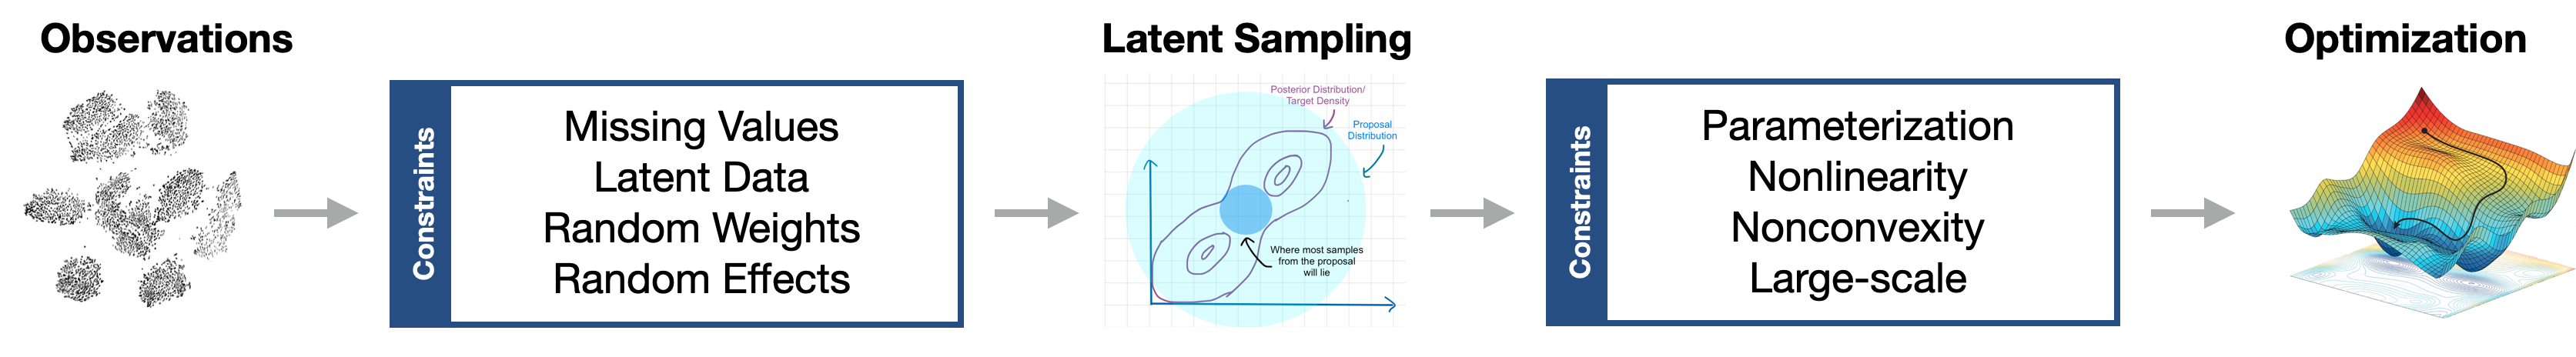
\includegraphics[width=\textwidth]{fig}
%\caption{fhzuz}
%\label{fig:myresearch}
\end{figure}

While my work provides \emph{novel} methods for particularly deep neural networks, one special case of the setting above, is when the input-output relationship of a phenomena is not completely characterized by the observations.
A set of latent variables is thus needed and the loss function accepts the latter as a third argument (the first two being the observations and the vector of parameters).

\noindent \textit{ Illustrative example of latent data model:} 
During clinical trials, the kinetics and dynamics of a drug being tested are modeled using nonlinear functions (or systems of ordinary differential equations) and observations from patients which comprise for instance their gender, height, concentration of the drug after injection.
While those observed covariates are necessary, they are not sufficient to describe well the biological pheonomena. 
A set of latent variables are used to quantify what can not be measured. 
In the special case of pharmacology, those latent variables describe the inter-individual variability among patients of a population (this is what makes us all different other than measurable signals). 
Therefore, the loss function, here the likelihood, is completed by simulations of those random effects and are then used to complete the observations before final optimization.

Thus, part of my research is at \emph{the intersection} of \textbf{sampling} and \textbf{optimization} bridging the gap between sampling methods such as Markov Chain Monte Carlo or Vational Inference and optimization method such as gradient based learning algorithms or maximum likelihood estimation.

My research has been published in top-tier conferences in machine learning such as NeurIPS, COLT, ICML and made the object of contribution in statistics Journal such as CSDA. I also received a collection of awards from those conferences and a Jacques Hadamard grant for a summer visit the Russian leading group in Bayesian Deep Learning called \emph{BayesGroup}.

Some of my work are now implemented in the commercial modeling and simulation software for drug development \emph{Lixoft} and in its open-source counter part \emph{saemix}.


\vspace{0.2in}


% ---------------------------------------------------Deep Learning: Training and Generalization-----------------------------------------------------------------------------------------
\textbf{\scalebox{1.6}{(a) Deep Learning: Training and Generalization}}
\vspace{0.2in}

A particular interest of mine lies in the practical training and theoretical understanding of deep neural networks, widely used for most learning tasks in the past decade.
Scaling, speeding and improving existing training algorithms is of utmost importance and drive most of my existing publications.


\vspace{0.15in}
\textbf{Training Acceleration} 
\vspace{0.08in}

\lipsum[35]


\vspace{0.15in}
\textbf{Decentralized Training} 
\vspace{0.08in}

\lipsum[35]

\vspace{0.15in}
\textbf{Towards Better Generalizaiton} 
\vspace{0.08in}

\lipsum[35]

\clearpage


% ---------------------------------------------------When Sampling meets Optimization-----------------------------------------------------------------------------------------

\textbf{\scalebox{1.6}{(b) When Sampling meets Optimization}}
\vspace{0.2in}

\lipsum[35]

\vspace{0.15in}
\textbf{Hierarchical Latent Structure Based Models} 
\vspace{0.08in}

\lipsum[35]


\vspace{0.15in}
\textbf{Two-level Stochastic Optimization Methods} 
\vspace{0.08in}

\lipsum[35]

\vspace{0.15in}
\textbf{MCMC Based Optimization} 
\vspace{0.08in}

\lipsum[35]

\newpage


% ---------------------------------------------------Future Research Directions-----------------------------------------------------------------------------------------
\textbf{\scalebox{1.6}{Future Research Directions}} 
\vspace{0.2in}

\lipsum[35]

\vspace{0.08in}
\paragraph{Energy Based Models.} \lipsum[35]

\vspace{0.08in}
\paragraph{Federated Learning.} \lipsum[35]

\vspace{0.08in}
\paragraph{Bayesian Deep Learning.} \lipsum[35]

\vspace{0.08in}
\paragraph{Stochastic Optimization for DNNs.} \lipsum[35]


\newpage


% ---------------------------------------------------References-----------------------------------------------------------------------------------------

\textbf{\scalebox{1.6}{References}}
\vspace{-0.3in}
\nocite{*}
\bibliography{references}

\end{document}
